\documentclass[letterpaper,12pt]{article}

%%%%%%%%%%%%%%%%%%%%%%%% Standard Packages %%%%%%%%%%%%%%%%%%%%%%%%%%%%%%%%%%%%%%%%%%
\usepackage{epsfig}
\usepackage{graphicx}
\usepackage{graphics}
\usepackage{amssymb}
\usepackage{amsmath}
\usepackage{mathrsfs}
\usepackage{fancyvrb}
\usepackage{caption}
\usepackage{comment}
\usepackage{fancyhdr}

%%%%%%%%%%%%%%%%%%%%%%%% Adapted from Sweave %%%%%%%%%%%%%%%%%%%%%%%%%%%%%%%%%%%%%%%%%

\DefineVerbatimEnvironment{Rcode}{Verbatim}{fontshape=sl, frame=single, 
  framesep=2mm, fontsize=\small, baselinestretch=.5}

%%%%%%%%%%%%%%%%%%%%%%%%%%%%%%%%%%%%%%%%%%%%%%%%%%%%%%%%%%%%%%%%%%%%%%%%%%%%%%%%%%%%%%

%%%%%%%%%%%%%%%%%%%%%%%% My macros (which of course are borrowed from a million ... %%
\def\argmax{\operatornamewithlimits{arg\,max}}
\def\argmin{\operatornamewithlimits{arg\,min}}


%%%%%%%%%%%%%%%%%%%%%%%% Page and Document Setup %%%%%%%%%%%%%%%%%%%%%%%%%%%%%%%%%%%%%
\addtolength{\oddsidemargin}{-0.875in}
\addtolength{\topmargin}{-0.875in}
\addtolength{\textwidth}{1.75in}
\addtolength{\textheight}{1.75in}

\captionsetup{margin=15pt,font=small,labelfont=bf}

\renewcommand{\topfraction}{0.9}        % max fraction of floats at top
\renewcommand{\bottomfraction}{0.8}     % max fraction of floats at bottom

% Parameters for TEXT pages (not float pages):
\setcounter{topnumber}{2}
\setcounter{bottomnumber}{2}
\setcounter{totalnumber}{4}             % 2 may work better
\setcounter{dbltopnumber}{2}            % for 2-column pages
\renewcommand{\dbltopfraction}{0.9}     % fit big float above 2-col. text
\renewcommand{\textfraction}{0.07}      % allow minimal text w. figs

% Parameters for FLOAT pages (not text pages):
\renewcommand{\floatpagefraction}{0.7}          % require fuller float pages

% N.B.: floatpagefraction MUST be less than topfraction !!
\renewcommand{\dblfloatpagefraction}{0.7}       % require fuller float pages


%%%%%%%%%%%%%%%%%%%%%%% options for sweave %%%%%%%%%%%%%%%%%%%%%%%%%%%%%%%%%%%%%%%%%%%%


%%%%%%%%%%%%%%%%%%%%%% headers and footers %%%%%%%%%%%%%%%%%%%%%%%%%%%%%%%%%%%%%%%%%%%%
\pagestyle{fancy} 
\renewcommand{\footrulewidth}{\headrulewidth}

%%%%%%%%%%%%%%%%%%%%%%%%% bibliography  %%%%%%%%%%%%%%%%%%%%%%%%%%%%%%%%%%%%%%%%%%%%%%%
\bibliographystyle{plainnat}


%%%%%%%%%%%%%%%%%%%%%%%%%%%%%%%%%%%%%%%%%%%%%%%%%%%%%%%%%%%%%%%%%%%%%%%%%%%%%%%%%%%%%%%
%%%%%%%%%%%%%%%%%%%%%%%%% Now Edit %%%%%%%%%%%%%%%%%%%%%%%%%%%%%%%%%%%%%%%%%%%%%%%%%%%%
%%%%%%%%%%%%%%%%%%%%%%%%%%%%%%%%%%%%%%%%%%%%%%%%%%%%%%%%%%%%%%%%%%%%%%%%%%%%%%%%%%%%%%%
\fancyhead[L]{\em Tu nombre}
\fancyhead[R]{\em templado}
\fancyfoot[L]{\em \today}
\fancyfoot[C]{}
\fancyfoot[R]{\em \thepage}


%%%%%%%%%%%%%%%%%%%%%%% opening %%%%%%%%%%%%%%%%%%%%%%%%%%%%%%%%%%%%
\title{Pon aqu� tu t�tulo}
\author{Tu nombre}

\usepackage{Sweave}
\begin{document}
\maketitle

%%%%% Pon lo que quieras aqu� %%%%
%%%%% Les muestro unos ejemplos %%%%
\begin{itemize}
  \item Un ejemplo de c�digo R:
\begin{Schunk}
\begin{Sinput}
> pop <- rep(0:1, c(10000 - 5600, 5600))
> res <- c()
> for (i in 1:1000) res[i] <- sum(sample(pop, 100))
> prop.test(mean(res), 100, conf.level = 0.95)
\end{Sinput}
\begin{Soutput}
	1-sample proportions test with continuity correction

data:  mean(res) out of 100, null probability 0.5 
X-squared = 1.2034, df = 1, p-value = 0.2726
alternative hypothesis: true p is not equal to 0.5 
95 percent confidence interval:
 0.4572113 0.6578373 
sample estimates:
      p 
0.55985 
\end{Soutput}
\end{Schunk}

  \item Un ejemplo de gr�fica:
  \begin{figure}[htbp] 
  \begin{centering}   
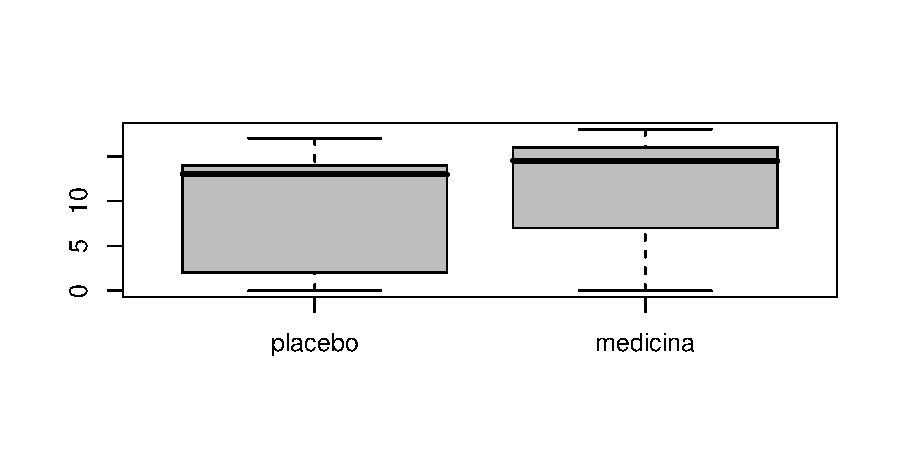
\includegraphics{templado-002}
  \end{centering} 
  \end{figure}
  
  \bigskip
  
  \item Un ejemplo de una enumeraci�n:
  \begin{enumerate}
    \item Primero 
	\item Segundo
	\item �ltimo
  \end{enumerate}

  \item Un ejemplo de una ecuaci�n:
  \begin{equation}
  y_i = \beta_0 + \beta_1x_i + \epsilon_i
  \end{equation}  

\end{itemize}


\end{document}
